


\begin{document}
Three different op amp topologies were provided as part of the lab. The chosen circuit can be seen in can be seen in Figure \ref{fig:default}.

\begin{figure}[H]
    \begin{center}
    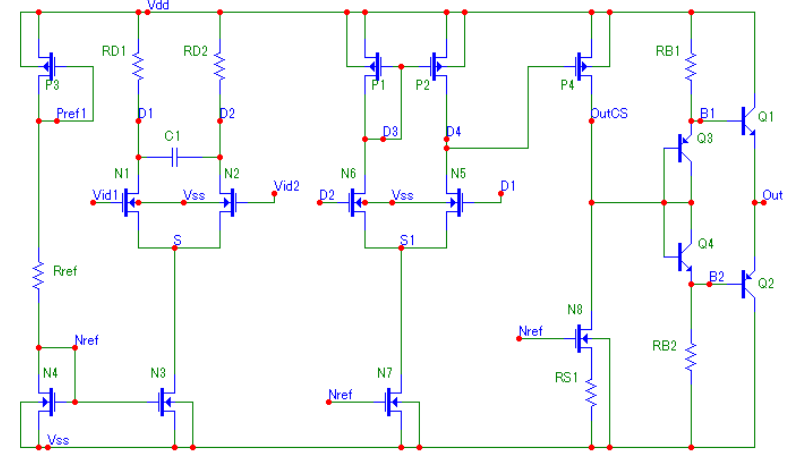
\includegraphics[scale=.85]{Simulations/default_circ.png}
    \caption{Generic schematic for chosen topology \cite{b2}}
    \label{fig:default}
    \end{center}
\end{figure}
This design was chosen due to the fact that every stage, with the exclusion of the output stage, was designed as part of a previous task. The stages can be broken down as such: a simple current mirror, a resistively loaded differential pair, an active loaded differential pair, an active load common source amplifier and finally a BJT amplifier output stage. The final simulated circuit can be seen in Figure \ref{fig:simcircuit}

\begin{figure}[H]
    \begin{center}
    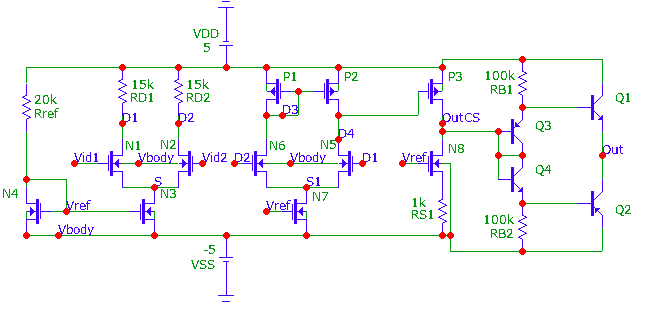
\includegraphics[scale=.85]{Simulations/simcircuit.png}
    \caption{Simulated op amp circuit}
    \label{fig:simcircuit}
    \end{center}
\end{figure}

The circuits will be simulated in MicroCap 11. The values for the components will initially be the values calculated in circuit development. The generic bias conditions for the ALD1106 and 1107 are summarized in Table \ref{tab:bias}. 

\begin{figure}[H]
	\begin{center}
		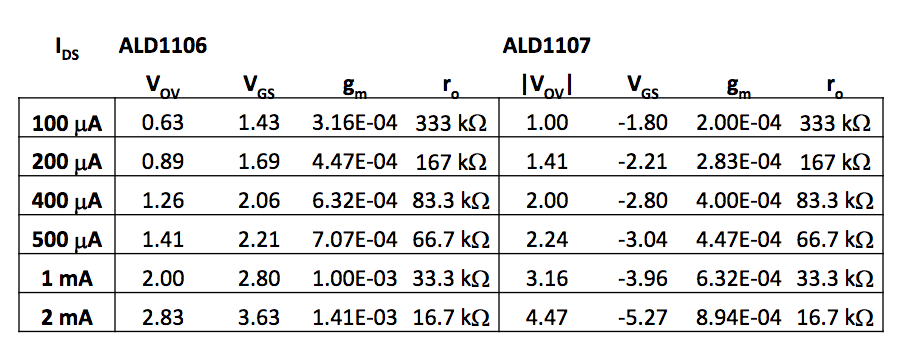
\includegraphics[scale=.85]{Simulations/nuribias.png}
		\caption{Typical ALD bias conditions \cite{b3}}
		\label{tab:bias}
	\end{center}
\end{figure}

Here the typical bias conditions for the constraining MOSFETs can be seen. For the purposes of this lab, the bias current of 400 $\mu$A was chosen.

\subsection{Resistively Loaded Differential Amplifier}

The resistively loaded amplifier stage requires a current mirror in order to generate the chosen bias current of 400 $\mu$A. This was achieved by applying Ohm's Law. The  V$_{gs}$ of the simple current mirror needs to be -3V. In order to  have the correct  current R$_{ref}$ was set to 20k$\Omega$. The simulated resistive load differential pair can be seen in Figure \ref{fig:ResLoadSim}.
\begin{figure}[H]
    \begin{center}
    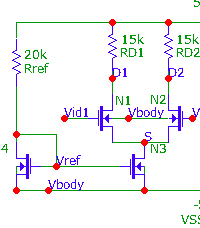
\includegraphics[scale=.85]{Simulations/simdiff.png}
    \caption{Simulated resistive load differential amplifier}
    \label{fig:ResLoadSim}
    \end{center}
\end{figure}

In addition, the current through the load resistors needs to be half of the bias current. As a result, the resistance values can be found by applying KVL, which leads to R$_{drain}$ of 15k$\Omega$.  The differential gain of the circuit can be found by Equation \ref{eq:Adsimresist} 
\begin{equation}\label{eq:Adsimresist}
A_d = g_m R_d,
\end{equation}

where g$_m$ is the transconductance of the amplifying NMOS and R$_d$ is the drain resistance and was calculated to be 16 dB. The output is double ended due to it feeding another amplifier stage. The simulated gain can be seen in  Figure \ref{fig:adsimresist}.


\begin{figure}[H]
    \begin{center}
    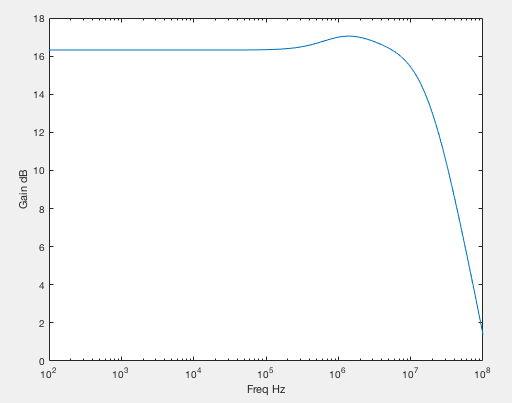
\includegraphics[scale=.30]{Simulations/gainfirststage.png}
    \caption{Simulated resistive load differential gain}
    \label{fig:adsimresist}
    \end{center}
\end{figure}
This was measured by performing an AC analysis in Microcap from 100Hz to 1MHz. This was performed by grounding one of the inputs whilest measuring the voltage differentially from the output nodes. The simulated value was marginally higher at 16.2 dB. The simulated phase can be seen in Figure  \ref{fig:firststagephase}.

\begin{figure}[H]
	\begin{center}
		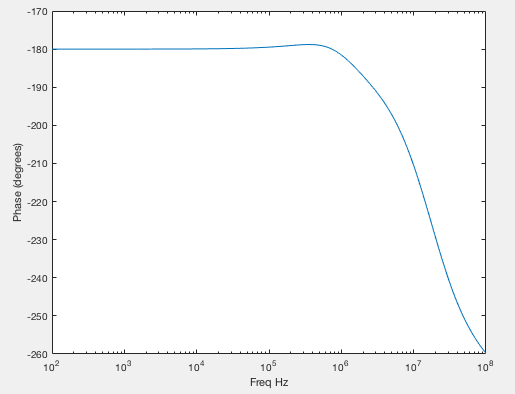
\includegraphics[scale=.30]{Simulations/phasefirststage.png}
		\caption{Simulated resistive load differential phase}
		\label{fig:firststagephase}.
	\end{center}
\end{figure}




\begin{figure}[H]
    \begin{subfigure}[b]{0.45\textwidth}
    \centering
    \includegraphics[scale=.30]{Simulations/Acm_resist_double.png}
    \caption{Simulated resistive load common mode gain}
    \label{fig:acmresistsim}
\end{subfigure}
    \hfill
     \begin{subfigure}[b]{0.45\textwidth}
    \centering
    \includegraphics[scale=.30]{Simulations/Acm_resist_double.png}
    \caption{Simulated CMRR resistive load}
    \label{fig:cmrrsimres}
\end{subfigure}
    \caption{Simulated Acm and CMRR resistive load}
    \label{fig:acmcmrrsim}
\end{figure} 

The Acm was measured by applying a differential signal to both inputs and measuring the differential outputs.
The simulation shows a constant Acm due to The Rss value being held constant by the simulation. The CMRR can be seen in Figure \ref{fig:cmrrsimres}. The CMRR if found by calculating the ratio of Ad to Acm and is seen to be similar to the calculated value.


\begin{table}[H]
\centering
\caption{Active load differential amplifier simulated results}
\label{my-label}
\begin{tabular}{|c|c|}
\hline
\multicolumn{2}{|c|}{\begin{tabular}[c]{@{}c@{}}Simulated resistively loaded \\ differential amplifier\end{tabular}} \\ \hline
Components/Nodes                                              & Values                                              \\ \hline
$V_{ref_1}$                                                   & -3.09 V                                               \\ \hline
$V_{ref_2}$                                                   & -.55 V                                                    \\ \hline
$I_{bias}$                                                    & 401 $\mu$A                                                    \\ \hline
$I_{ref_1}$                                                   &  199 $\mu$A                                                   \\ \hline
$I_{ref_2}$                                                   & 202 $\mu$A                                                    \\ \hline
\end{tabular}
\end{table}




\subsection{Active load differential amplifier}
The active load amplifier schematic is shown in Figure \ref{fig:ActiveLoadSim}. Rref did not need changing for simulations.

\begin{figure}[H]
    \begin{center}
    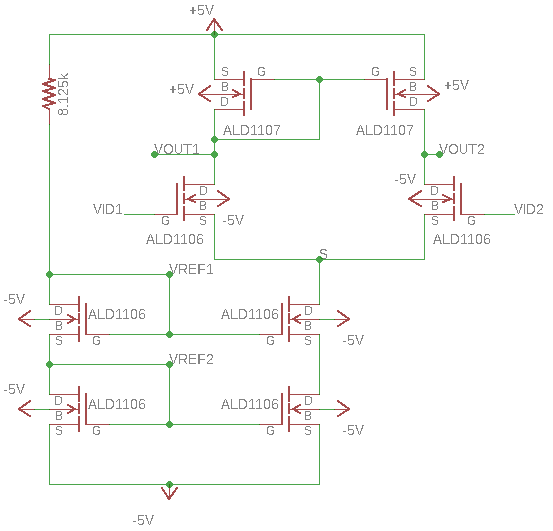
\includegraphics[scale=.85]{Simulations/ActiveLoadedSimulated.png}
    \caption{Simulated active load differential amplifier}
    \label{fig:ActiveLoadSim}
    \end{center}
\end{figure}'

The differential gain for the active load can be seen in Figure \ref{fig:activeAdsim}.


\begin{figure}[H]
    \begin{center}
    \includegraphics[scale=.30]{Simulations/Ad_active_double.png}
    \caption{Simulated active load differential gain}
    \label{fig:activeAdsim}
    \end{center}
\end{figure}
This simulation was performed in the same manner as the resistive load. The differential gain is found to be much high than resistive load. The common mode gain was simulated in the same manner as the resitive load, with a differential signal being applied at both inputs with the voltage at the outputs being measured differentially. The Acm and CMRR can be seen in Figure \ref{fig:acmcmrrsimactive}.



\begin{figure}[H]
    \begin{subfigure}[b]{0.45\textwidth}
    \centering
    \includegraphics[scale=.30]{Simulations/Acm_active_double.png}
    \caption{Simulated active load common mode gain}
    \label{fig:activeAcsim}
    \end{subfigure}
    \hfill
    \begin{subfigure}[b]{0.45\textwidth}
    \centering
    \includegraphics[scale=.30]{Simulations/CMRR_active_double.png}
    \caption{Simulated active load CMRR}
    \label{fig:activeCMRRsim}
\end{subfigure}
    \caption{Simulated Acm and CMRR active load}
    \label{fig:acmcmrrsimactive}
\end{figure} 


Proceeding from the common mode gain, the CMRR can be was calculated in Matlab and was found to be constant. The summary of simulated active load values can be seen in Table \ref{tab:simactiveload}.



\begin{table}[H]
\centering
\caption{Active load differential amplifier simulated results}
\label{tab:simactiveload}
\begin{tabular}{|c|c|}
\hline
\multicolumn{2}{|c|}{\begin{tabular}[c]{@{}c@{}}Simulated active loaded \\ differential amplifer\end{tabular}} \\ \hline
Components/Nodes                                              & Values                                              \\ \hline
$V_{ref_1}$                                                   & -3.07 V                                                    \\ \hline
$V_{ref_2}$                                                   & -.51 V                                                    \\ \hline
$I_{bias}$                                                    & 401 $\mu$A                                                    \\ \hline
$I_{ref_1}$                                                   & 200 $\mu$A                                                    \\ \hline
$I_{ref_2}$                                                   & 199 $\mu$A                                                    \\ \hline
\end{tabular}
\end{table}

The DC values were found by performing DC analysis in Microcap. The values are extremely comparable to the calculated values.




\end{document}